\documentclass{beamer}    %slidestop=title in up-left corner (with "slidescentered" centered); compress=navigation bars as small as possible

%\usepackage[ugm]{mathdesign} %use Garamond font

%gets rid of bottom navigation bars and puts slide numbers right bottom
\setbeamertemplate{footline}[frame number]{}

%alternative footer: name, institute, page number
%\setbeamertemplate{footline}
%{%
%  \leavevmode%
%  \hbox{\begin{beamercolorbox}[wd=.5\paperwidth,ht=2.5ex,dp=1.125ex,leftskip=.3cm plus1fill,rightskip=.3cm]{author in head/foot}%
%    \usebeamerfont{author in head/foot}\insertshortauthor
%  \end{beamercolorbox}%
%  \begin{beamercolorbox}[wd=.5\paperwidth,ht=2.5ex,dp=1.125ex,leftskip=.3cm,rightskip=.3cm plus1fil]{title in head/foot}%
%    \usebeamerfont{title in head/foot}\insertshortinstitute \hfill \insertframenumber \,/\,\inserttotalframenumber
%  \end{beamercolorbox}}%
%  \vskip0pt%
%}

%gets rid of navigation symbols
\setbeamertemplate{navigation symbols}{}


%%complete themes (not recommended)
%%\usetheme{Madrid}             %"Berkeley":lhs navigation bar; 1st alternative: "Madrid" without a navigation bar but with a footer including name (institution), title, date page numbering (but then \institute{Univ. ...}); 2nd alternative: defaults without all the extras; 3rd alternative "Dresden": two bottom lines)
%%"Dresden is possibly easy to adapt to UvT colors
%instead of using a complete theme inner and outer themes can be specified in isolation
%inner theme:
\useinnertheme{rounded} %actually not necessary but nice for theorem boxes etc. but enumerate listings look a bit stupid! Alternative: default = just comment it out
%outer themes:
%\useoutertheme[subsection=false,footline=authorinstitutetitlepage]{miniframes} %other options for footer see beamer user guide p. 153


%%complete color themes: (ok but inner outer styles below are better)
%%\usecolortheme{albatross}    % background is colored (in blue) in albatross; the option [overlystylish] installs a background canva which is definitely too stylish for an economics department
%%\usecolortheme{seagull}   %for greyscale (black and white)
%%default is not bad!!!

%alternative to complete color schemes one can define an inner and outer color scheme
%inner color themes
%\usecolortheme{orchid} %deep color in box(theorem etc.) background fits with outer color scheme "whale"
\usecolortheme{rose} % less aggressive slight grey shading background (in boxes/theorems etc.) fits nicely with outer color scheme \usecolortheme{seahorse}
%outer color theme
\usecolortheme{dolphin}   %alternative to seahorse: "whale" but only if inner scheme is "orchid"
%
%\usefonttheme{structurebold}       %titles, headlines, foodlines and sidebars are bold

\usepackage{amsmath, eurosym, textcomp, graphicx, amsthm, amssymb,amsfonts, natbib, url, xcolor, tikz, subfig}

\usepackage[english]{babel} %English language if Koma script classes are used (Bibliography instead of Inhaltsverzeichnis..)
\usepackage[latin1]{inputenc}
\usepackage[T1]{fontenc} %Encoding 
\usepackage{ae,aecompl}%avoids the problem of faint or hardly printable output
\usepackage{pdfsync} %in supporting pdf viewers, this enables forward and inverse search
\synctex=1

\usepackage{sgame} %Osborne's packages to draw games
\usepackage{hyperref}
%\usepackage[all]{hypcap}


% \usepackage{comment}
% \newcommand{\com}{\comment}
% \newcommand{\ecom}{\endcomment}

%\usepackage{ngerman}
\setlength {\parindent}{0cm}
\newcommand {\bi}{\begin{itemize}}
\newcommand {\ei}{\end{itemize}}
\newcommand{\be}{\begin{enumerate}}
\newcommand{\ee}{\end{enumerate}}
\newcommand{\Ra}{\Rightarrow}
\newcommand{\ra}{\rightarrow}
\newcommand{\Lra}{\Leftrightarrow}
\newcommand{\del}{\partial}
\newcommand{\bea}{\begin{eqnarray*}}
\newcommand{\eea}{\end{eqnarray*}}
\newcommand{\less}{<}
\newcommand{\great}{>}
\newcommand{\vbar}{|}
\renewcommand{\Re}{\mathbb{R}}
\renewcommand{\P}{\mathcal{P}}

\theoremstyle{plain}
\newtheorem{prop}{Proposition}
%\newtheorem{theorem}{Theorem}
\newtheorem{assumption}{Assumption}
%\newtheorem{lemma}{Lemma}
\newtheorem{proposition}{Proposition}
\newtheorem{observation}{Observation}
\newtheorem{result}{Result}
%\newtheorem{corollary}{Corollary}
\theoremstyle{definition}
\newtheorem{ex}{Example}
\newtheorem{exercise}{Exercise}
%\newtheorem{definition}{Definition}

%\setlength{\parskip}{1.5ex plus 0.5ex minus 0.5ex}
\author{Christoph Schottm\"uller}
\institute{University of Copenhagen}
\title{Game Theory\\ Perfect equilibrium in extensive form games}

\date{}

\newcommand{\fr}{\frame[allowframebreaks]}
\newcommand{\ft}{\frametitle}

\newcommand{\backupbegin}{
   \newcounter{framenumberappendix}
   \setcounter{framenumberappendix}{\value{framenumber}}
}
\newcommand{\backupend}{
   \addtocounter{framenumberappendix}{-\value{framenumber}}
   \addtocounter{framenumber}{\value{framenumberappendix}}
}

\begin{document}
\maketitle
% \section[Outline]{}
% \frame{\ft{Outline}\tableofcontents}



\fr{\ft{Reminder: Game trees and information sets}

\begin{ex}
Information sets in a game tree are indicated by (dashed) lines between the nodes that build the information set.
  \begin{figure}[h]
\centering
% First, set the overall layout of the tree
% You might need to play with these sizes to ensure nothing overlaps.
\tikzstyle{level 1}=[level distance=1.5cm, sibling distance=3.5cm]
\tikzstyle{level 2}=[level distance=1.5cm, sibling distance=3.5cm]
\tikzstyle{level 3}=[level distance=1.5cm, sibling distance=2cm]
\tikzstyle{level 4}=[level distance=1.5cm, sibling distance=1.5cm]
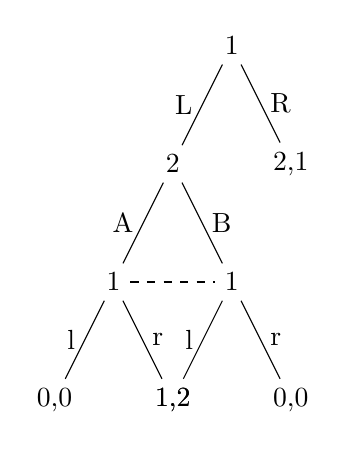
\begin{tikzpicture}
%Start with the parent node, and slowly build out the tree
% with each "child" representing a new level of the diagram
% each "node" represents a labelled (or unlabeled if you 
% want) node in the diagram.
\node{1}
    child{
             node{2}
             child{
               node(a){1}
                  child{
               node{0,0}
               edge from parent
               node[left]{l}
               }
             child{
               node{1,2}
               edge from parent
               node[right]{r}
               }
               edge from parent
               node[left]{A}
               }
             child{
               node(b){1}
                  child{
               node{1,2}
               edge from parent
               node[left]{l}
               }
             child{
               node{0,0}
               edge from parent
               node[right]{r}
               }
               edge from parent
               node[right]{B}
               }
           edge from parent
           node[left]{L}
           }
    child{
         node{2,1}
         edge from parent
         node[right]{R}
         };
\draw [dashed](a)--(b);
\end{tikzpicture}
%\caption{extensive form game with imperfect information}
%\label{fig:ext_game_imperf_info}
\end{figure}

\end{ex}

% \begin{definition}
%   An \textbf{extensive game} consists of the following components
%  \begin{itemize}
%   \item set $N$ of players
%   \item set $H$ of sequences (denoting possible  histories)
%     \begin{itemize}
%     \item empty sequence is in $H$ (this is the initial/starting node)
%     \item if $(a^k)_{k=1\dots K}$ is in $H$, then $(a^k)_{k=1\dots L}$ is also in $H$ for all $L\less K$ (each history is connected with the initial node)
%     \item if $(a^k)_{k=1\dots K}$ is in $H$ for any integer $K$, then $(a^k)_{k=1}^\infty$ is also in $H$
%     \end{itemize}
%     a history $(a^k)_{k=1\dots K}$ is \emph{terminal} if it is an infinite sequence or if there is no $a^{K+1}$ such that $(a^k)_{k=1\dots K+1}$ is in $H$. The set of terminal histories is denoted by $Z$.  The set of actions available after the non-terminal history $h$ is denoted by $A(h)=\{a: (h,a)\in H\}$.
% \end{itemize}
% \end{definition}
% \begin{definition}[continued]
% \begin{itemize}  
% \item a player function $P$ that assigns each non-terminal history a member of $N\cup \{c\}$ (the player who has to take an action or ``chance'' for random moves by ``nature'')
%   \item a functon $f_c$ that associates with each $h$ where $P(h)=c$ a probability measure on $A(h)$ ($f_c(a\vbar h)$ is probability that $a$ occurs after history $h$); each such probability measure is independent of the other probability measures
%   \item for each player $i\in N$ a partition $\mathcal{I}_i$ of $\{h:P(h)=i\}$ with the property that $A(h)=A(h')$ whenever $h$ and $h'$ are in the same partition member (each $I_i\in\mathcal{I}_i$ is called an \emph{information set} of player $i$)
%   \item for each player a utility function $u_i$ on lotteries over $Z$
%   \end{itemize}
% \end{definition}

% \begin{itemize}
% \item %$\langle N,H,P,f_c,(\mathcal{I}_i)\rangle$ is extensive game form 
% $\langle N,H,P,f_c,(\mathcal{I}_i), (u_i)\rangle$ is extensive game
% \item why are preferences defined over ``lotteries on Z''?
% % \item equivalent definition through game tree: information sets consist then of nodes at which the same player acts

% % \item that's why $A(h)$ has to be the same for all histories in one information set (otherwise player could infer which history was played)
% % \item a player can, of course, have a belief about which of the histories in the information set was played (in example above, player believed $a$ is played in the vowel info-set as this is equilibrium action)

% \end{itemize}



\begin{ex}
  Here a game tree with a chance move.
 \begin{figure}[h]
\centering
% First, set the overall layout of the tree
% You might need to play with these sizes to ensure nothing overlaps.
\tikzstyle{level 1}=[level distance=1.5cm, sibling distance=6cm]
\tikzstyle{level 2}=[level distance=1.5cm, sibling distance=2.5cm]
\tikzstyle{level 3}=[level distance=1.5cm, sibling distance=2cm]
\tikzstyle{level 4}=[level distance=1.5cm, sibling distance=1.5cm]
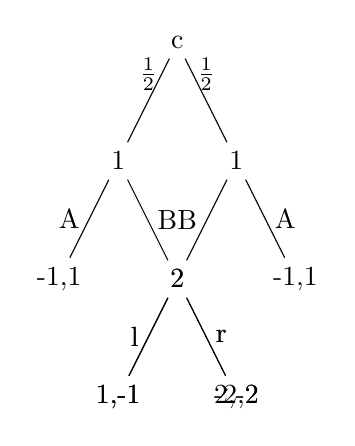
\begin{tikzpicture}
%Start with the parent node, and slowly build out the tree
% with each "child" representing a new level of the diagram
% each "node" represents a labelled (or unlabeled if you 
% want) node in the diagram.
\node{c}
    child{
             node{1}
             child{
               node(a){-1,1}
               edge from parent
               node[left]{A}
               }
             child{
               node(b){2}
                  child{
               node{1,-1}
               edge from parent
               node[left]{l}
               }
             child{
               node{2,-2}
               edge from parent
               node[right]{r}
               }
               edge from parent
               node[right]{B}
               }
           edge from parent
           node[left,above]{$\frac{1}{2}$}
           }
    child{
         node{1}
           child{
               node(c){2}
                  child{
               node{1,-1}
               edge from parent
               node[left]{l}
               }
             child{
               node{-2,2}
               edge from parent
               node[right]{r}
               }
               edge from parent
               node[left]{B}
               }
             child{
               node(d){-1,1}
               edge from parent
               node[right]{A}
               }
         edge from parent
         node[right,above]{$\frac{1}{2}$}
         };
\draw [dashed](c)--(b);
\end{tikzpicture}
%\caption{extensive form game with imperfect information and chance move}
%\label{fig:ext_game_imperf_info_chance}
\end{figure}
% Chance moves with probabiltiy $1/2$ either left or right. Player 1 is informed about the chance move while player 2 is not.
\end{ex}

% \begin{definition}
%   A \textbf{pure strategy} of player $i\in N$ is a function that assigns to each information set $I_i\in \mathcal{I}_i$ an action in $A(I_i)$.
% \end{definition}

% What are the pure strategies of player 1 in the first example game?
}

\section{Intermezzo: Imperfect Recall}

\fr{\ft{Intermezzo: Imperfect recall}

   \begin{figure}[h]
\centering
% First, set the overall layout of the tree
% You might need to play with these sizes to ensure nothing overlaps.
\tikzstyle{level 1}=[level distance=1.5cm, sibling distance=5cm]
\tikzstyle{level 2}=[level distance=1.5cm, sibling distance=2cm]
\tikzstyle{level 3}=[level distance=1.5cm, sibling distance=2cm]
\tikzstyle{level 4}=[level distance=1.5cm, sibling distance=1.5cm]

\begin{tikzpicture}[scale=0.5]
%Start with the parent node, and slowly build out the tree
% with each "child" representing a new level of the diagram
% each "node" represents a labelled (or unlabeled if you 
% want) node in the diagram.
\node(a){1}
    child{
             node(b){1}
             child{
               node{}
               edge from parent
               node[left]{}
               }
             child{
               node{}
               edge from parent
               node[right]{}
               }
           edge from parent
           node[left,above]{}
           }
    child{
         node{}
         edge from parent
         node[right,above]{}
         };
%\draw[dashed] (a) to [out=100,in=190] (b);
\draw[dashed, bend right] (a) to (b);
\end{tikzpicture}
\quad
\begin{tikzpicture}[scale=0.5]
%Start with the parent node, and slowly build out the tree
% with each "child" representing a new level of the diagram
% each "node" represents a labelled (or unlabeled if you 
% want) node in the diagram.
\node{c}
    child{
             node{1}
             child{
               node(a){}
               edge from parent
               node[left]{}
               }
             child{
               node(b){1}
                  child{
               node{}
               edge from parent
               node[left]{}
               }
             child{
               node{}
               edge from parent
               node[right]{}
               }
               edge from parent
               node[right]{}
               }
           edge from parent
           node[left,above]{}
           }
    child{
         node{1}
           child{
               node(c){1}
                  child{
               node{}
               edge from parent
               node[left]{}
               }
             child{
               node{}
               edge from parent
               node[right]{}
               }
               edge from parent
               node[left]{}
               }
             child{
               node(d){}
               edge from parent
               node[right]{}
               }
         edge from parent
         node[right,above]{}
         };
\draw [dashed](c)--(b);
\end{tikzpicture}
\quad
\begin{tikzpicture}[scale=0.5]
%Start with the parent node, and slowly build out the tree
% with each "child" representing a new level of the diagram
% each "node" represents a labelled (or unlabeled if you 
% want) node in the diagram.
\node(a){1}
    child{
             node(b){1}
             child{
               node{}
               edge from parent
               node[left]{}
               }
             child{
               node{}
               edge from parent
               node[right]{}
               }
           edge from parent
           node[left,above]{}
           }
    child{
         node(c){1}
          child{
               node{}
               edge from parent
               node[left]{}
               }
             child{
               node{}
               edge from parent
               node[right]{}
               }
         edge from parent
         node[right,above]{}
         };
%\draw[dashed] (a) to [out=100,in=190] (b);
\draw[dashed] (c) to (b);
\end{tikzpicture}
\caption{extensive form games with imperfect recall}
%\label{fig:ext_game_imperf_recall}
\end{figure}

\framebreak

Interpretation 1:
\begin{itemize}
\item left game: P1 forgets whether he moved already or not
\item right game: P1 forgets what he previously knew (which move chance played)
\item bottom game: P1 forgets what he previously did
\end{itemize}
Interpretation 2:
\begin{itemize}
\item information set represents the information about history that is inherent in the game, i.e. the information the game provides to the player when it is his move
\item the player can refine this information by inferences% , i.e. the player actually remembers what he did/knew and therefore in the three games above he has the information needed when he has to act; it is just not provided by the game but by his inference
\item under this interpretation the expression ``imperfect recall'' is a bit misleading
\end{itemize}

\framebreak

how many pure strategies does P1 have in each of the three games on the previous slide?:
\begin{itemize}
\item left game: %only 1 info-set $\Ra$ two pure strategies (say $L$ or $R$)
\item right game: %P1 has 3 info sets with 2 possible actions each $\Ra$  8 pure strategies
\item bottom game: %P1 has 2 info sets with two actions each $\Ra$ 4 pure strategies
\end{itemize}


\begin{itemize}
\item imperfect recall is a bit troublesome (at least in the first
  interpretation) 
\item we talk now a bit about it and then ``forget it''
\item  to illustrate the problems consider the sleeping beauty example
\end{itemize}

\begin{ex}[sleeping beauty]
  \begin{itemize}
  \item  on Sunday the sleeping beauty  is put to sleep
  \item a fair coin is then tossed
    \begin{itemize}
    \item if heads:
      \begin{itemize}
      \item beauty is wakened and interviewed on Monday, and then the
        experiment ends
      \end{itemize}

    \item  if tails:
      \begin{itemize}
      \item beauty is wakened and interviewed on Monday and Tuesday
      \item when she is put to sleep again on Monday, she is given a
        dose of an amnesia-inducing drug that ensures she cannot
        remember her previous awakening
      \item experiment ends after she is interviewed on Tuesday
      \end{itemize}
    \end{itemize}
    Any time Sleeping Beauty is wakened and interviewed, she is
    asked, ``What probability do you assign to the event that the
    coin landed heads?''\\
What should she answer?% \emph{(from wikipedia)}
  \end{itemize}
\end{ex}
% \begin{ex}[sleeping beauty, continued]
% two positions:
% \begin{itemize}
% \item probability is $1/3$: if the experiment was repeated 1000 times, one expects 500 head and 500 tails; hence, the beauty is woken up 1500 times; one third of these times heads ocurred
% \item probability is $1/2$: the belief was $1/2$ at the beginning; being woken up does not reveal any new information (it happens no matter how the coin falls); hence, there is no reason to update the belief
% \end{itemize}
% \end{ex}

}

\section{Behavioral strategies}
\fr{\ft{Mixed and behavioral strategies}
\begin{definition}
  % A \textbf{mixed strategy} of player $i$ in an extensive game $\langle N, H, P,f_c,(\mathcal{I}_i),(u_i)\rangle$ is a probability measure over the set of pure strategies.\\
Let $\mathcal{I}_i$ be the set of all information sets in which player $i$ has to act and denote the actions from which player $i$ has to choose in information set $I_i$ by $A(I_i)$. \\ A \textbf{behavioral strategy} of player $i$ is a collection $(\beta_i(I_i))_{I_i\in \mathcal{I}_i}$ of independent probability measures where $\beta_i(I_i)$ is a probability measure over $A(I_i)$.
\end{definition}

\begin{itemize}
% \item mixed strategy mixes over pure strategy, pure strategy is a complete plan of action prescribing an action at every information set a player might have to act
\item behavioral strategy prescribes a mix over actions at every information set a player might have to act
\framebreak
\item first example game:
  \begin{itemize}
  %\item  can you given an example of a mixed strategy of P1?% P1 has 4 pure strategies (L,l), (L,r), (R,l), (R,r); a mixed strategy is a probability distribution over these four pure strategies 
  \item can you give an example of a behavioral strategy of P1?% a behavioral strategy consists of two probabiltiy distributions: one over L and R; the other over r and l
  \end{itemize}
\end{itemize}
 \begin{figure}[h]
\centering
% First, set the overall layout of the tree
% You might need to play with these sizes to ensure nothing overlaps.
\tikzstyle{level 1}=[level distance=1.5cm, sibling distance=3.5cm]
\tikzstyle{level 2}=[level distance=1.5cm, sibling distance=3.5cm]
\tikzstyle{level 3}=[level distance=1.5cm, sibling distance=2cm]
\tikzstyle{level 4}=[level distance=1.5cm, sibling distance=1.5cm]
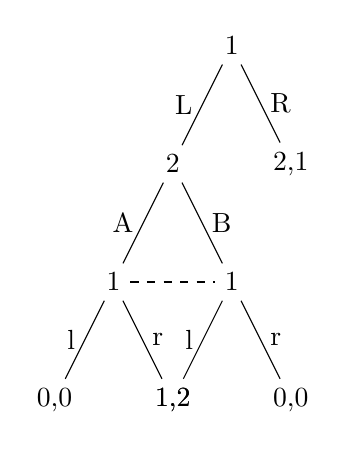
\begin{tikzpicture}
%Start with the parent node, and slowly build out the tree
% with each "child" representing a new level of the diagram
% each "node" represents a labelled (or unlabeled if you 
% want) node in the diagram.
\node{1}
    child{
             node{2}
             child{
               node(a){1}
                  child{
               node{0,0}
               edge from parent
               node[left]{l}
               }
             child{
               node{1,2}
               edge from parent
               node[right]{r}
               }
               edge from parent
               node[left]{A}
               }
             child{
               node(b){1}
                  child{
               node{1,2}
               edge from parent
               node[left]{l}
               }
             child{
               node{0,0}
               edge from parent
               node[right]{r}
               }
               edge from parent
               node[right]{B}
               }
           edge from parent
           node[left]{L}
           }
    child{
         node{2,1}
         edge from parent
         node[right]{R}
         };
\draw [dashed](a)--(b);
\end{tikzpicture}
%\caption{extensive form game with imperfect information}
%\label{fig:ext_game_imperf_info}
\end{figure}
% \framebreak
% \item mixed strategies are in line with mixing in strategic games but behavioral strategies are often more convenient to use in extensive games
% \item recall that a mixed strategy could be interpreted as a belief held by other players
%   \begin{itemize}
%   \item mixed strategy: conjecture of others over $i$'s complete game plan
%   \item behavioral strategy: collection of independent beliefs about what action player $i$ would choose after some history
%   \end{itemize}

% \framebreak
% \item  Behavioral or mixed strategies? Does it matter?
% \end{itemize}

% \begin{definition}
%   For any strategy profile $\sigma=(\sigma_i)_{i\in N}$ (of mixed or behavioral strategies), we define the \textbf{outcome $O(\sigma)$ of $\sigma$} to be the probability distribution over the terminal histories that results if each player $i$ uses $\sigma_i$.
% \end{definition}


% \begin{definition}
%   Two strategies (mixed or behavioral) are \textbf{outcome equivalent} if for every collection of pure strategies of the other players the two strategies induce the same outcome.
% \end{definition}

% %\framebreak

% \begin{proposition}
%   In finite extensive games with perfect recall, for any mixed strategy there is an outcome equivalent behavioral strategy and for every behavioral strategy there is an outcome equivalent mixed strategy.
% \end{proposition}
% \textbf{Proof. }(\emph{(sketch)})
% \begin{itemize}
% \item Take a behavioral strategy $\beta_i$ and let us define an
%   outcome equivalent mixed strategy% , i.e. we have to assign a
%   % probability to each pure strategy $s_i$ (and these probabilities
%   % have to sum up to 1). Recall that each pure strategy $s_i$ assigns
%   % each inforamtion set $I_i\in\mathcal{I}_i$ one available action
%   % $a\in A(I_i)$.
%   \begin{itemize}
%   \item Assign each pure strategy $s_i$ the probability $\Pi_{I_i\in
%       \mathcal{I}_i}\beta_i(I_i)(s_i(I_i))$. The mixed strategy
%     $\sigma_i$ defined this way is outcome equivalent to $\beta_i$\dots
%   \end{itemize}
% % Take any collection of pure strategies $s_{-i}$ and an
% %   arbitrary terminal history $h$ that is conistent with
% %   $s_{-i}$. Summing the probabilities under $\sigma_i$ of $h$ over all
% %   $s_i$ consistent with $h$ gives by the definition of $\sigma_i$
% %   $\Pi_{I_i\in X_i(h)}\beta_i(I_i)(s_i(I_i))$which is the probability
% %   under $\beta_i$ (as $s_{-i}$ is consistent with $h$ the
% %   probabilities of the other players are 1).  \par
% \item  Take a mixed strategy $\sigma_i$
%   \begin{itemize}
%   \item $\pi_i(h)$ denotes the probability that player $i$ plays actions consistent with $h$ under $\sigma_i$
%   % \item. Let $h$ and $h'$ be histories in the same information set $I_i\in\mathcal{I}_i$. Perfect recall implies that $\pi_i(h)=\pi_i(h')$ (player $i$ took the same actions at every info set preceding $I_i$ otherwise $h$ and $h'$ would not be in the same info set). In any pure strategy the action $a$ is taken after $h$ if and only if it is also take after $h'$ (both are in the same info set). Hence, $\pi_i(h,a)=\pi_i(h',a)$. Therefore, we can
% \item let $h$ be a history leading to the information set $I_i$ and let $a$ be an action player $i$ can choose at this information set
% \item    define $\beta_i(I_i)(a)=\pi_i(h,a)/\pi_i(h)$ if $\pi_i(h)\great 0$% . Clearly, $\sum_{a\in A(h)}b_i(I_i)(a)=1$.
%  % \\
%   \item  $\beta_i$ and $\sigma_i$ are outcome
%     equivalent\dots%  Take some pure strategy collection $s_{-i}$ and some
%     % terminal history $h$. If $h$ is inconsistent with $s_{-i}$ or
%     % $\sigma_i$, clearly $O(h)=0$ also with $\beta_i$. If $h$ is
%     % consitent with $s_{-i}$ and $\sigma_i$, the probability of outcome
%     % $h$ under $\beta_i$ is the product of $\pi_i(h',a)/\pi_i(h')$ over
%     % all subhistories $(h',a)$ of $h$ which is the probability of $h$
%     % under $\sigma_i$ (note that this is multiplying conditional
%     % probabilities, e.g. prob of playing $a^1$ times prob of playing
%     % $a^2$ given $a^1$ was played which equals the unconditional prob
%     % of prob of $a^2$ \dots).
%   \end{itemize}

% \end{itemize}
% \qed



% \begin{ex}
%   Take our previous example:
%   \begin{itemize}
%   \item Take the mixed strategy of P1  $(L,l)$ with probability $0.2$, $(L,r)$ with $0.1$, $(R,l)$ with $0.4$ and $(R,r)$ with $0.3$\par
%  What is the corresponding behavioral strategy?% \\
%     % $\beta_1(\emptyset)(L)=0.3$ and $\beta_1(\emptyset)(R)=0.7$ and
%     % $\beta_1(\{(L,A),(L,B)\})(l)=2/3$ and
%     % $\beta_1(\{(L,A),(L,B)\})(r)=1/3$\par
%   \item  P1 uses the behavioral strategy $\beta_1(\emptyset)(L)=0.6$ and $\beta_1(\emptyset)(R)=0.4$ and $\beta_1(\{(L,A),(L,B)\})(l)=0.2$ and $\beta_1(\{(L,A),(L,B)\})(r)=0.8$.\par
%  What is mixed strategy?% \\
%     % $(L,l)$ with $0.12$ and $(L,r)$ with $0.48$ and $(R,l)$ with
%     % $0.08$ and $(R,r)$ with $0.32$
%   \end{itemize}

% \end{ex}

% \begin{itemize}
% \item Nash equilibrium in mixed strategies is defined as before as a profile $\sigma$ of mixed strategies such that for each $i\in N$ and for every mixed strategy $\sigma_i'$ of player $i$
% $$u_i(O(\sigma_{-i},\sigma_i))\geq u_i(O(\sigma_{-i},\sigma_i'))$$
% \item alternative definition is that each player has only pure strategies in the support of $\sigma_i$ which are a best response to $\sigma_{-i}$
% \item Nash equilibrium in behavioral strategies is defined analogously, i.e. $\beta_i$ is a best response to the behavioral strategies of the other players for all $i$ or
% $$u_i(O(\beta_{-i},\beta_i))\geq u_i(O(\beta_{-i},\beta_i'))$$
% \item with perfect recall Nash equilibria in behavioral and mixed strategies coincide
% % \item without perfect recall not the case: take left game on slide 20 and say that payoff after $(l,l)$ and $(r)$ is 0 but after $(l,r)$ the payoff is 1. Every mixed strategy is optimal and gives payoff 0. The optimal behavioral strategy mixes $1/2$, $1/2$ and gives payoff $1/4$.
% \end{itemize}
}

\section{Perfect equilibrium}
\fr{\ft{Perfect equilibrium}
 \begin{figure}[h]
\centering
% First, set the overall layout of the tree
% You might need to play with these sizes to ensure nothing overlaps.
\tikzstyle{level 1}=[level distance=1.5cm, sibling distance=6cm]
\tikzstyle{level 2}=[level distance=1.5cm, sibling distance=2.5cm]
\tikzstyle{level 3}=[level distance=1.5cm, sibling distance=2cm]
\tikzstyle{level 4}=[level distance=1.5cm, sibling distance=1.5cm]
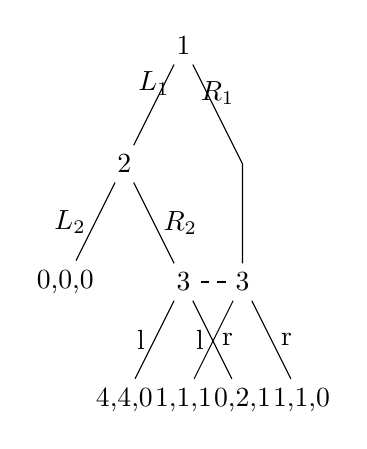
\begin{tikzpicture}
%Start with the parent node, and slowly build out the tree
% with each "child" representing a new level of the diagram
% each "node" represents a labelled (or unlabeled if you 
% want) node in the diagram.
\node{1}
    child{
             node{2}
             child{
               node{0,0,0}
             edge from parent
             node[left]{$L_2$}}
             child{
               node(b){3}
                  child{
               node{4,4,0}
               edge from parent
               node[left]{l}
               }
             child{
               node{0,2,1}
               edge from parent
               node[right]{r}
               }
                edge from parent
                node[right]{$R_2$}
               }
           edge from parent
           node[left,above]{$L_1$}
           }
    child{
           child{
               node(c){3}
                  child{
               node{1,1,1}
               edge from parent
               node[left]{l}
               }
             child{
               node{1,1,0}
               edge from parent
               node[right]{r}
               }
               }
         edge from parent
         node[right,above]{$R_1$}
         };
\draw [dashed](c)--(b);
\end{tikzpicture}
\caption{Selten's example}
\label{fig:selten_ex}
\end{figure}
How should rational play look in this example? \\
\begin{itemize}
\item no proper subgames $\Ra$ every NE is SPNE
\item ($R_1,L_2,l$) is NE but is it reasonable?
\item would player 2 play $L_2$ if he was called upon to act? % No (whatever 3 does any outcome after $R_2$ is better)!
\item will player 1 then play $R_1$? % he knows that player 2 will play $R_2$ and as player 3 does not know what is going on, he will stick to his equilibrium strategy $l$. Hence, No!
\item ($R_1,L_2,l$) is NE but not self enforcing!
\item a self enforcing equilibrium:
  \begin{itemize}
  % \item idea: P2 has to play $R_2$; if P1 plays $L_1$ for sure P3 plays $r$ and P1 wants to deviate; hence mixing of P1; mixing determines equilibrium beliefs of P3; mix such that P3 is indifferent between as mixing by P3 is the only way to make P1 indifferent
  \item P1 plays $L_1$ and $R_1$ with prob 1/2
   \item P2 plays $R_2$
   \item P3 plays 1/4 $l$ and 3/4 $r$
  \end{itemize}
\end{itemize}

\framebreak

\begin{itemize}
\item Problem with ($R_1,L_2,l$): information set that is reached with zero probability when equilibrium strategies are played
\item in corresponding strategic form: P2 plays weakly dominated strategy % ($L_2$ and $R_2$ are equally good if P1 plays $R_1$ but if not $L_2$ is worse than $R_2$)
\item recall Selten's idea of trembling hand perfect equilibrium: % (each player makes mistakes with small probability),
  %then 
all info sets are reached with positive probability when trembling %and no zero probability info set $\Ra$ no problem
\item reminder: trembling hand perfection (roughly): a perfect equilibrium is a NE that is a limit of completely mixed equilibria
\end{itemize}

\framebreak

%Another problem can be seen in the following game
\begin{figure}
\centering
\tikzstyle{level 1}=[level distance=1.5cm, sibling distance=3cm]
\tikzstyle{level 2}=[level distance=1.5cm, sibling distance=2.5cm]
\tikzstyle{level 3}=[level distance=1.5cm, sibling distance=2cm]
\begin{tikzpicture}
%Start with the parent node, and slowly build out the tree
% with each "child" representing a new level of the diagram
% each "node" represents a labelled (or unlabeled if you 
% want) node in the diagram.
\node(a){1}
    child{
             node(b){2}
             child{
               node{1}
                child{node{3,3}
                  edge from parent 
                  node[left]{l}}
                  child{node{2,0}
                  edge from parent
                  node[right]{r}}
               edge from parent
               node[left]{a}
               }
             child{
               node{0,2}
               edge from parent
               node[right]{b}
               }
           edge from parent
           node[left,above]{L}
           }
    child{
         node(c){1,1}
         edge from parent
         node[right,above]{R}
         };
\end{tikzpicture}
\caption{Why agent strategic form?}
\label{fig:why_agent_strat_form}
\end{figure}

What is the SPNE? Is there another trembling hand perfect NE in the corresponding strategic form?

\framebreak

\begin{itemize}
\item one SPNE: ((L,l),a)
\item  ((R,r),b): % is trembling hand perfect as all strategies, i.e. (L,l) and b, are rational given that the other player plays his equilibrium strategy with high probability; the problem is that
  P1 does not consider that he himself could make the mistake of playing L instead of R%; if he considered this possibility l would be better than r
\item $\Ra$ agent strategic form: for a given extensive form game G the agent strategic form
  \begin{itemize}
  \item has a player $ih$ for each information set $h$ of each player $i$ in $G$
  \item the actions of $ih$ correspond to the actions of $i$ at $h$ in $G$
  \item the payoff function of $ih$ is equal to the payoff function of $i$ in $G$
  \item is a strategic form game!
  \end{itemize}
\item idea is fully decentralized decision making where each player delegates decision making at any information set to one agent
% \item the agent strategic form of the game above (figure \ref{fig:why_agent_strat_form}) has three agents; one for P2 and two for P1

\begin{figure}[h]
\centering
\tikzstyle{level 1}=[level distance=1.5cm, sibling distance=3cm]
\tikzstyle{level 2}=[level distance=1.5cm, sibling distance=2.5cm]
\tikzstyle{level 3}=[level distance=1.5cm, sibling distance=2cm]
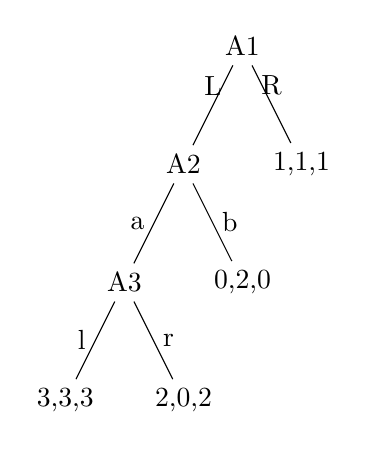
\begin{tikzpicture}
%Start with the parent node, and slowly build out the tree
% with each "child" representing a new level of the diagram
% each "node" represents a labelled (or unlabeled if you 
% want) node in the diagram.
\node(a){A1}
    child{
             node(b){A2}
             child{
               node{A3}
                child{node{3,3,3}
                  edge from parent 
                  node[left]{l}}
                  child{node{2,0,2}
                  edge from parent
                  node[right]{r}}
               edge from parent
               node[left]{a}
               }
             child{
               node{0,2,0}
               edge from parent
               node[right]{b}
               }
           edge from parent
           node[left,above]{L}
           }
    child{
         node(c){1,1,1}
         edge from parent
         node[right,above]{R}
         };
\end{tikzpicture}
\caption{getting to the agent strategic form}
\label{fig:agent_strat_form}
\end{figure}

\begin{table}[h]
\centering
 \begin{game}{2}{2}[][][l]
   &a&b\\
L &3,3,3&0,2,0\\
R&1,1,1&1,1,1
\end{game}
\quad
\begin{game}{2}{2}[][][r]
   &a&b\\
L &2,0,2&0,2,0\\
R&1,1,1&1,1,1
\end{game}
\caption{agent strategic form}
\label{tab:agent_strat_form}
\end{table}
\item strategies in the agent strategic form are similar to behavioral strategies in the extensive form game
\end{itemize} 

\framebreak

\begin{definition}
  A (trembling hand) \textbf{perfect equilibrium of an extensive form
  game} $G$ is a perfect equilibrium in the agent strategic
  form of $G$.
\end{definition}
\begin{itemize}
\item we already showed that every finite strategic form game has a perfect equilibrium this gives directly
  \begin{corollary}
    There exists a perfect equilibrium in every finite extensive form game.
  \end{corollary}

\framebreak

\item let's go back to Selten's example: % in any perturbed game P1 plays $L_1$ with some probability; 
 % hence 
  \begin{itemize}
  \item P2's best action in each perturbed game is $R_2$ and therefore
    no equilibrium including $L_2$ is perfect
  \item is the self-enforcing equilibrium in Selten's example perfect?\\
    Yes: let the equilibrium strategies in the fully mixed perturbed
    game be
    \begin{itemize}
    \item P1 plays $L_1$ with prob $1/(2-\varepsilon )$ and $R_1$ with prob $(1-\varepsilon )/(2-\varepsilon )$
    \item P2 plays $L_2$ with prob $\varepsilon$ and $R_2$ with prob
      $1-\varepsilon$
    \item P3 plays $l$ with prob $1/(4*(1-\varepsilon ))$ and $r$ with prob $(3-4\varepsilon)/(4*(1-\varepsilon ))$
    \end{itemize}
  \end{itemize}
\end{itemize}

% \begin{ex}
% \begin{figure}[h]
% \centering
% \tikzstyle{level 1}=[level distance=1.5cm, sibling distance=3.5cm]
% \tikzstyle{level 2}=[level distance=1.5cm, sibling distance=2cm]
% \tikzstyle{level 3}=[level distance=1.5cm, sibling distance=1.5cm]
%   \begin{tikzpicture}[scale=0.9]
% %Start with the parent node, and slowly build out the tree
% % with each "child" representing a new level of the diagram
% % each "node" represents a labelled (or unlabeled if you 
% % want) node in the diagram.
% \node(a){1}
%     child{
%              node(b){2}
%              child{
%                node{0,0}
%                edge from parent
%                node[left]{L}
%                }
%              child{
%                node{1,1}
%                edge from parent
%                node[right]{R}
%                }
%            edge from parent
%            node[left,above]{L}
%            }
%     child{
%          node(c){1}
%           child{
%                node{0,0}
%                edge from parent
%                node[left]{l}
%                }
%              child{
%                node{1,2}
%                edge from parent
%                node[right]{r}
%                }
%          edge from parent
%          node[right,above]{R}
%          };
% %\draw[dashed] (a) to [out=100,in=190] (b);
% \end{tikzpicture}
% \caption{example perfect equilibrium}\label{fig:some_ex_perf_eq}
% \end{figure}
%  %The corresponding agent strategic form is 
% \vspace*{-1.3cm}
%  \begin{table}[h]
%    \centering
%    \begin{game}{2}{2}[][][l]
%      & L&R\\
% L &0,0,0&1,1,1\\
% R&0,0,0&0,0,0
%    \end{game}
% \qquad
%    \begin{game}{2}{2}[][][r]
%      & L&R\\
% L &0,0,0&1,1,1\\
% R&1,2,1&1,2,1
%    \end{game}
%    \caption{agent strategic form}
%    \label{tab:ex_perf_eq_ext}
%  \end{table}
% \vspace*{-0.8cm}
% \end{ex}

% \framebreak

% \begin{ex}[continued]
%   \begin{itemize}
%   \item ((L,r),R) is a perfect equilibrium % . To
%     % see this let player 1b tremble with with probability $\varepsilon$
%     % and player 1a and 2 with prob $\varepsilon^2$.\par
%    \item % Let us use the coalescing moves principal and reduce the original
%     % game to one where P1 chooses between L, l and r in his first
%     % move. The (agent) strategic form of this game is
%    the intital game seems equivalent to a game where P1 moves only once and has the actions $L,l,r$
 

% \begin{table}[h]
%   \centering
%   \begin{game}{3}{2}
%     &L&R\\
% L &0,0&1,1 \\
% l &0,0&0,0 \\
% r &1,2&1,2
%   \end{game}
%   \caption{(agent) strategic form after coalescing moves}
%   \label{tab:perf_eq_coalesc_moves}
% \end{table}
%  only trembling hand perfect equilibrium is (r,R) %  To see this, P1 prefers r to any action if P2 completely mixes and P2 prefers R to L whenever P1 completely mixes.  Hence, perfect equilibrium is not robust to coalescing moves.
%  \end{itemize}
% \end{ex}

% \begin{itemize}
% \item perfect equilibrium is not robust to ``coalescing moves''
% \end{itemize}
}

\frame{\ft{Review questions}
  \begin{itemize}
  \item What is imperfect recall and what problems does it cause?
  \item What is a behavioral strategy?
  \item Why do we define perfect equilibrium in extensive form games through the ``agent strategic form'' instead of using the usual normal form representation of the extensive form game?
  \item How is perfect equilibrium defined in extensive form games?
  \end{itemize}
reading: perfect equilibrium: MSZ 7.3.2 or OR 12.5.2; on extensive form games${}^{(*)}$: OR 11.1 and 11.4
}

\fr{\ft{Exercises}
  \begin{enumerate}
  \item Bob has to drive home from work. To get home he has to go straight at the first crossroad and turn right at the second crossroad. The two crossroads look excatly identical and Bob is ``absent minded'': Whenever he arrives at a crossroad he does not know whether it is the first or the second crossroad. Assume that his payoff from coming home is 1 while his payoff from going wrong is 0. What should Bob do?
 \item Write down the corresponding normal form game of the game below. Show that there are four Nash equilibria and show that (CD,L) is a perfect equilibrium in the normal form game. Write down the agent strategic form and show that (CD,L) is not a perfect equilibrium in the agent strategic form. Find a perfect equilibrium of the game.

\begin{figure}[h]
\centering
% First, set the overall layout of the tree
% You might need to play with these sizes to ensure nothing overlaps.
\tikzstyle{level 1}=[level distance=2cm, sibling distance=3.5cm]
\tikzstyle{level 2}=[level distance=1.5cm, sibling distance=2cm]
\tikzstyle{level 3}=[level distance=1.5cm, sibling distance=2cm]
\tikzstyle{level 4}=[level distance=1.5cm, sibling distance=1cm]
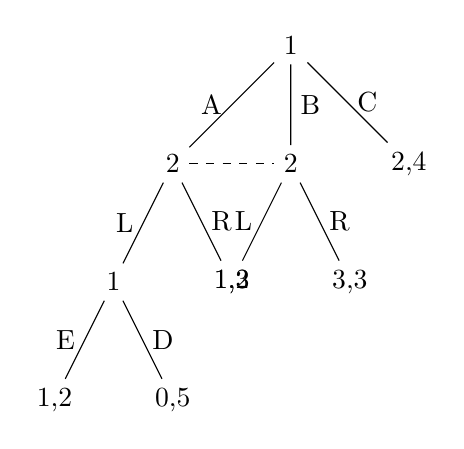
\begin{tikzpicture}
%Start with the parent node, and slowly build out the tree
% with each "child" representing a new level of the diagram
% each "node" represents a labelled (or unlabeled if you 
% want) node in the diagram.
\node {1}
    child{
      node(na){2}
       child{
             node{1}
             child{
             node{1,2}
             edge from parent
             node[left]{E}
              }
              child{
             node{0,5}
             edge from parent
             node[right]{D}
              }
           edge from parent
           node[left]{L}
           }
       child{
         node{1,3}
         edge from parent
         node[right]{R}
         }
      edge from parent
      node[left]{A}
     }
  child{
    node(nb){2}
    child{
             node{1,2}
             edge from parent
             node[left]{L}
              }
              child{
             node{3,3}
             edge from parent
             node[right]{R}
              }
    edge from parent
    node[right]{B}
    }
  child{
     node{2,4}
     edge from parent
    node[right]{ C} 
     };
\draw[dashed] (na) to (nb);
\end{tikzpicture}
\end{figure} 
  \end{enumerate}
}

\end{document}